\documentclass[journal,12pt,twocolumn]{IEEEtran}
\usepackage{./report_macros}

\begin{document}
\vspace{3cm}
\title{CS5760 Assignment Report: Differential Cryptanalysis of a Custom 6-Round DES}
\author{Gautam Singh\\CS21BTECH11018}
\maketitle
\tableofcontents

\section{Introduction}
\label{sec:intro}
This report describes the differential cryptanalysis of a custom 6 round DES
using weakened S boxes. It documents the implementation details as well as the
characteristics used for cryptanalysis of DES. The codes are implemented in
Python and prerequisites are documented in the attached README.

\section{S Boxes}
\label{sec:s-box}
S boxes have been implemented using the Python class \texttt{SBoxDES} in the
file \texttt{util.py}. These S boxes take as input the 4 by 16 S box and
implement methods to compute the output of the S box and generate the
differential distribution table (DDT). The DDT itself is computed by counting
the frequency of the input-output XOR pair over all possible input pairs. DDTs
are formatted and written to a user specified text file.

\section{Characteristics}
\label{sec:char}

High probability differential trails across multiple rounds need to be generated
to create a useful characteristic for cryptanalysis. In particular, to implement
the six-round 3R-attack in \cite{bihamDifferentialCryptanalysisDESlike1991} with
few encryptions, we require to generate a three round characteristic with high
probability to boost the signal-to-noise ratio and reduce the number of pairs
needed. 

To achieve a high signal-to-noise ratio, we constrain ourselves to inputs and
outputs to the DES \(F\) function which have as few bits set to activate fewer S
boxes. This is because activating many S boxes would lower the characteristic
probability since it would contain the product of many quantities less than 1.
Further, the expansion function \(E\) of DES duplicates set bit in positions
\(0, 1 \bmod 4\). Hence, we mainly consider inputs \(4_x, 8_x, 12_x\) to S
boxes, since the corresponding input bits appear only once in the expansion.

From the DDT of S7, we see that \(04_x \rightarrow 2_x\) with probability
\(\frac{24}{64} = \frac{3}{8}\). From the DDT of S6, we see that \(08_x
\rightarrow 4_x\) with probability \(\frac{22}{64} = \frac{11}{32}\). These are
two ``desirable'' input-output XOR pairs in the context of the discussion above.

Each of these pairs forms their own characteristic as shown in
\autoref{fig:char1} and \autoref{fig:char2}.

\begin{figure}[!ht]
    \centering
    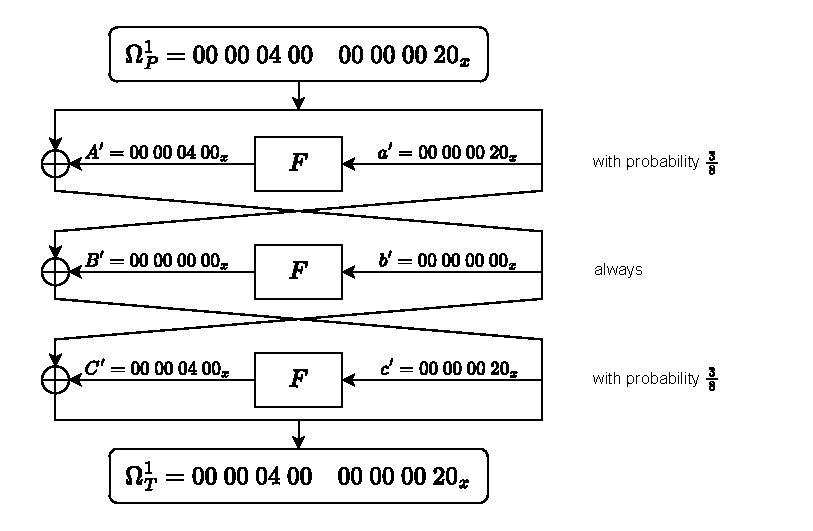
\includegraphics[width=\columnwidth]{images/char1.pdf}
    \caption{Characteristic used for cryptanalysis with probability \(\frac{9}{64}\).}
    \label{fig:char1}
\end{figure}

\begin{figure}[!ht]
    \centering
    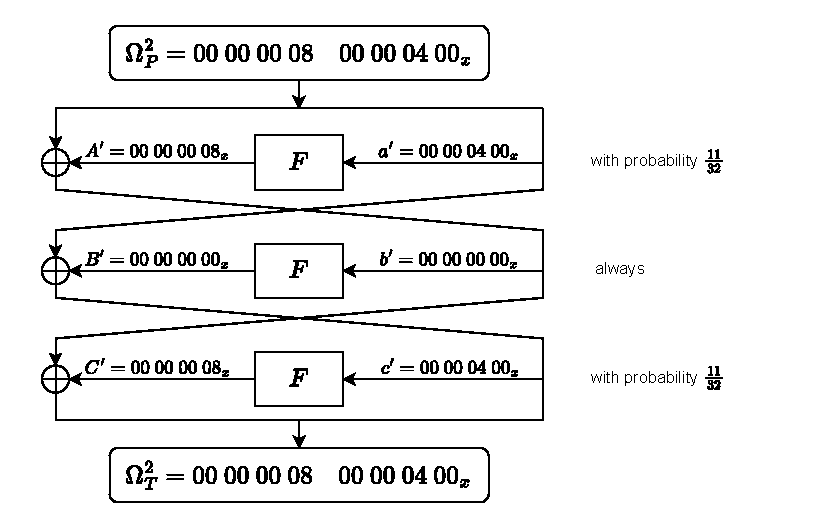
\includegraphics[width=\columnwidth]{images/char2.pdf}
    \caption{Characteristic used for cryptanalysis with probability \(\frac{121}{1024}\).}
    \label{fig:char2}
\end{figure}

\section{Cryptanalysis}
\label{sec:recovery}

In this section, we describe the various methods and data structures used to
cryptanalyze DES reduced to 6 rounds. In our implementation, we largely treat
plaintexts and ciphertexts as 64-bit integers for fast bit manipulations. Our
implementation is reproducible since the random seed is set. Notice that
changing the random seed may result in the key not being recovered since the
plaintexts generated suggested multiple key values.

\subsection{Cache}
\label{subsec:cache}

We implement a cache to query the oracle and store the responses. Suitable
manipulations between integers and 64-bit bitstrings are done before and after
the query. The ciphertext is extracted from the received HTML response which is
parsed using \texttt{BeautifulSoup4}.

\subsection{Graph}
\label{subsec:graph}

We implement the clique method described in
\cite{bihamDifferentialCryptanalysisDESlike1991} to significantly boost the
signal-to-noise ratio. Masks for each S box are stored in a \texttt{Node}
object. The clique algorithm itself is implemented as a naive backtracking
algorithm. It is fast in practice due to the randomly chosen plaintexts which
reduce the size of the maximal clique greatly, thereby pruning the search space.

\subsection{Summary and Complexity Analysis}
\label{subsec:summary}

In summary, the attack proceeds as follows.

\begin{enumerate}
    \item Generate quartets and their corresponding ciphertexts.
    \item For each characteristic, run the clique algorithm to find suggested
    key values. Ensure that both characteristics suggest the same key values.
    This gives us the value of \(K6\).
    \item Brute force on the remaining 8 key bits to get the entire master key,
    verifying each possible key against a few randomly chosen plaintext
    encryptions.
\end{enumerate}

Suppose \(q\) quartets are used and \(p\) randomly chosen plaintexts are used
for verification. Then, this attack takes \(p + 4q\) oracle queries. In our
implementation, \(p = 20\) and \(q = 50\) for a total of 220 encryptions.

\section{Results}
\label{sec:results}

For the given DES implementation and weak S boxes, the output of the key
recovery program \texttt{recover.py} is shown in \autoref{lst:output}.

\begin{listing}[!ht]
    \centering
    \inputminted[breaklines,breakanywhere,breaksymbol=,breakanywheresymbolpre=]{text}{artefacts/output.txt}
    \caption{Output of key recovery program.}
    \label{lst:output}
\end{listing}

\bibliography{references.bib}

\end{document}
